% Results-section LaTeX fragment for the TRACE-RAG paper.
% Required packages in the main paper preamble:
% \usepackage{booktabs}
% \usepackage{graphicx}
%
% All reported values use the curated n=200 summary tables and positive
% showcase assets generated in this repository.

\section{Experimental Results}
\label{sec:results}

\subsection{Main Results}
\label{sec:main-results}

TRACE-RAG delivers its clearest gains on MuSiQue, the more complex multi-hop QA
benchmark. Table~\ref{tab:musique-main-results} compares the strongest
non-TRACE-RAG baseline with the best TRACE-RAG configuration for each model backbone.
Across DeepSeek, GPT-4o-mini, and Gemini, the best TRACE-RAG configuration improves
over the strongest baseline by an average of 4.33 points in accuracy, 4.33
points in exact match, and 5.84 points in F1. The gains are largest for Gemini,
where TRACE-RAG tog+bm25 improves F1 from 20.99 to 30.26.

\begin{table}[t]
\centering
\small
\begin{tabular}{llrrrr}
\toprule
Model & Best TRACE-RAG vs. baseline & $\Delta$Acc. & $\Delta$EM & $\Delta$F1 & TRACE-RAG F1 \\
\midrule
DeepSeek & TRACE-RAG tog+bm25 vs. ToG & +0.50 & +0.50 & +1.38 & 31.44 \\
GPT-4o-mini & TRACE-RAG hippo+bm25 vs. HippoRAG & +2.50 & +5.00 & +6.87 & 31.77 \\
Gemini & TRACE-RAG tog+bm25 vs. RAPTOR & +10.00 & +7.50 & +9.27 & 30.26 \\
\midrule
Average & -- & +4.33 & +4.33 & +5.84 & -- \\
\bottomrule
\end{tabular}
\caption{Main MuSiQue results. Each row compares the best TRACE-RAG configuration
with the strongest non-TRACE-RAG baseline for the same model backbone.}
\label{tab:musique-main-results}
\end{table}

PopQA shows a more mixed pattern, which is expected for a simpler factoid QA
setting where sparse retrieval is already strong. TRACE-RAG remains competitive:
it slightly improves F1 over the strongest baseline for DeepSeek and
GPT-4o-mini, but is slightly below the strongest Gemini baseline. We therefore
use PopQA as robustness evidence rather than as the central performance claim.

\begin{table}[t]
\centering
\small
\begin{tabular}{llrrrr}
\toprule
Model & Best TRACE-RAG vs. baseline & $\Delta$Acc. & $\Delta$EM & $\Delta$F1 & TRACE-RAG F1 \\
\midrule
DeepSeek & TRACE-RAG hippo+bm25 vs. BM25 & +0.00 & -0.50 & +0.92 & 29.78 \\
GPT-4o-mini & TRACE-RAG hippo+bm25 vs. BM25 & -1.00 & -0.50 & +0.20 & 29.06 \\
Gemini & TRACE-RAG hippo+bm25 vs. HippoRAG & -2.00 & +0.00 & -0.35 & 27.50 \\
\bottomrule
\end{tabular}
\caption{PopQA robustness results. TRACE-RAG is competitive on factoid QA but does
not uniformly exceed the strongest baseline for every model backbone.}
\label{tab:popqa-robustness-results}
\end{table}

\begin{figure}[t]
\centering
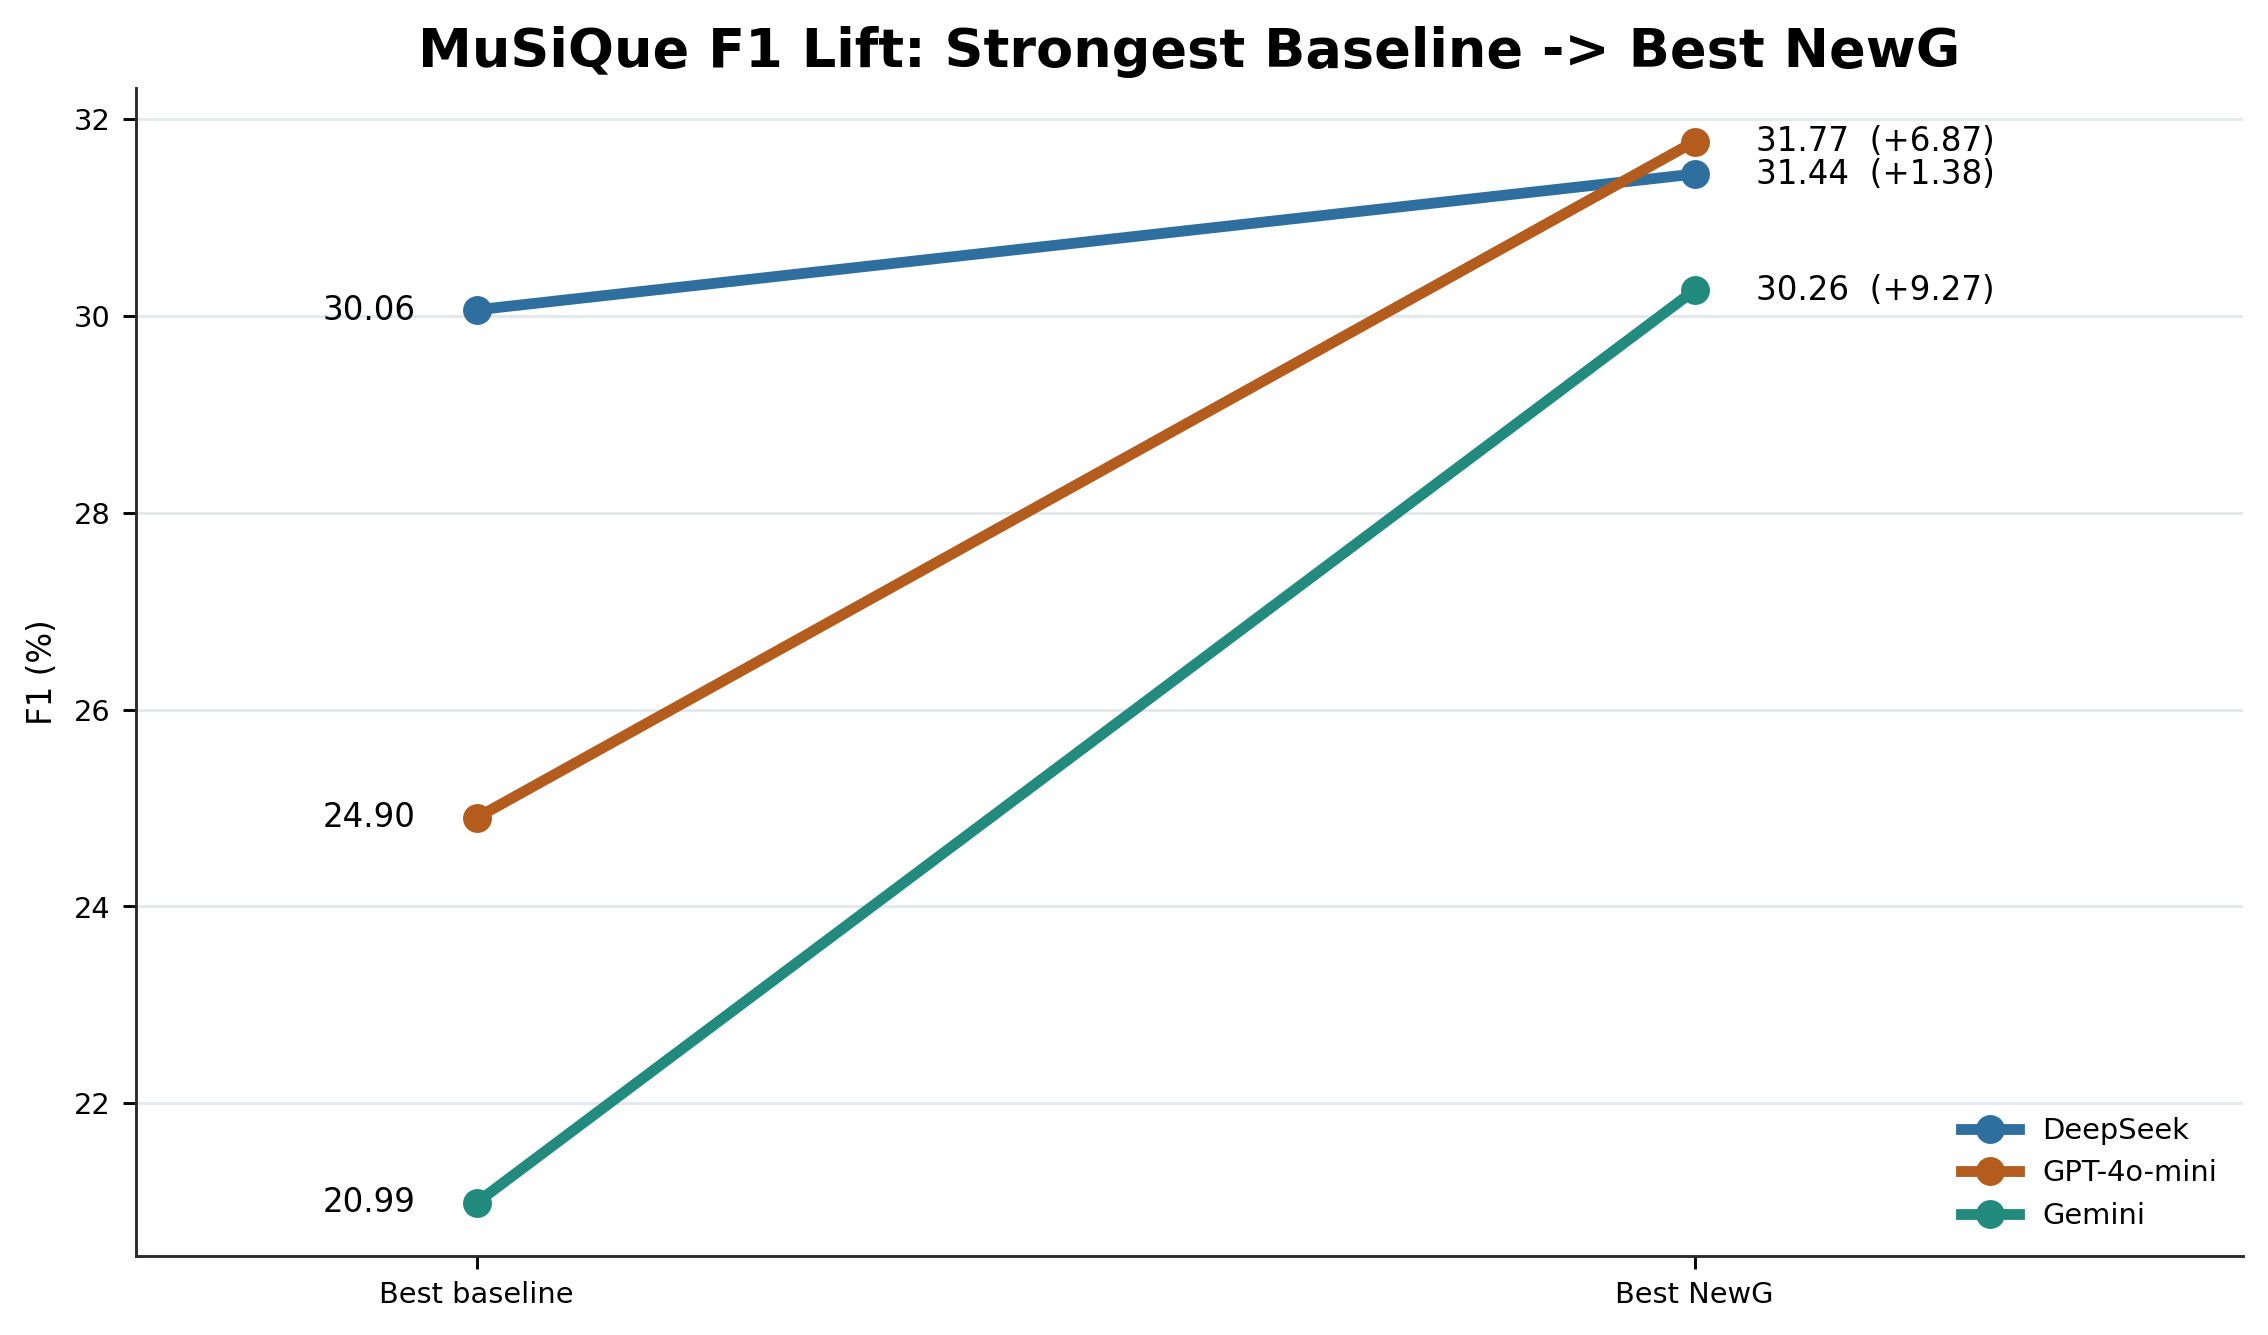
\includegraphics[width=\linewidth]{figures/positive_showcase/panel_musique_best_f1_lift.png}
\caption{TRACE-RAG improves over the strongest non-TRACE-RAG baseline on MuSiQue across
all three model backbones. Bars show the F1 lift for the best TRACE-RAG
configuration relative to the strongest baseline.}
\label{fig:musique-main-gains}
\end{figure}

\begin{figure}[t]
\centering
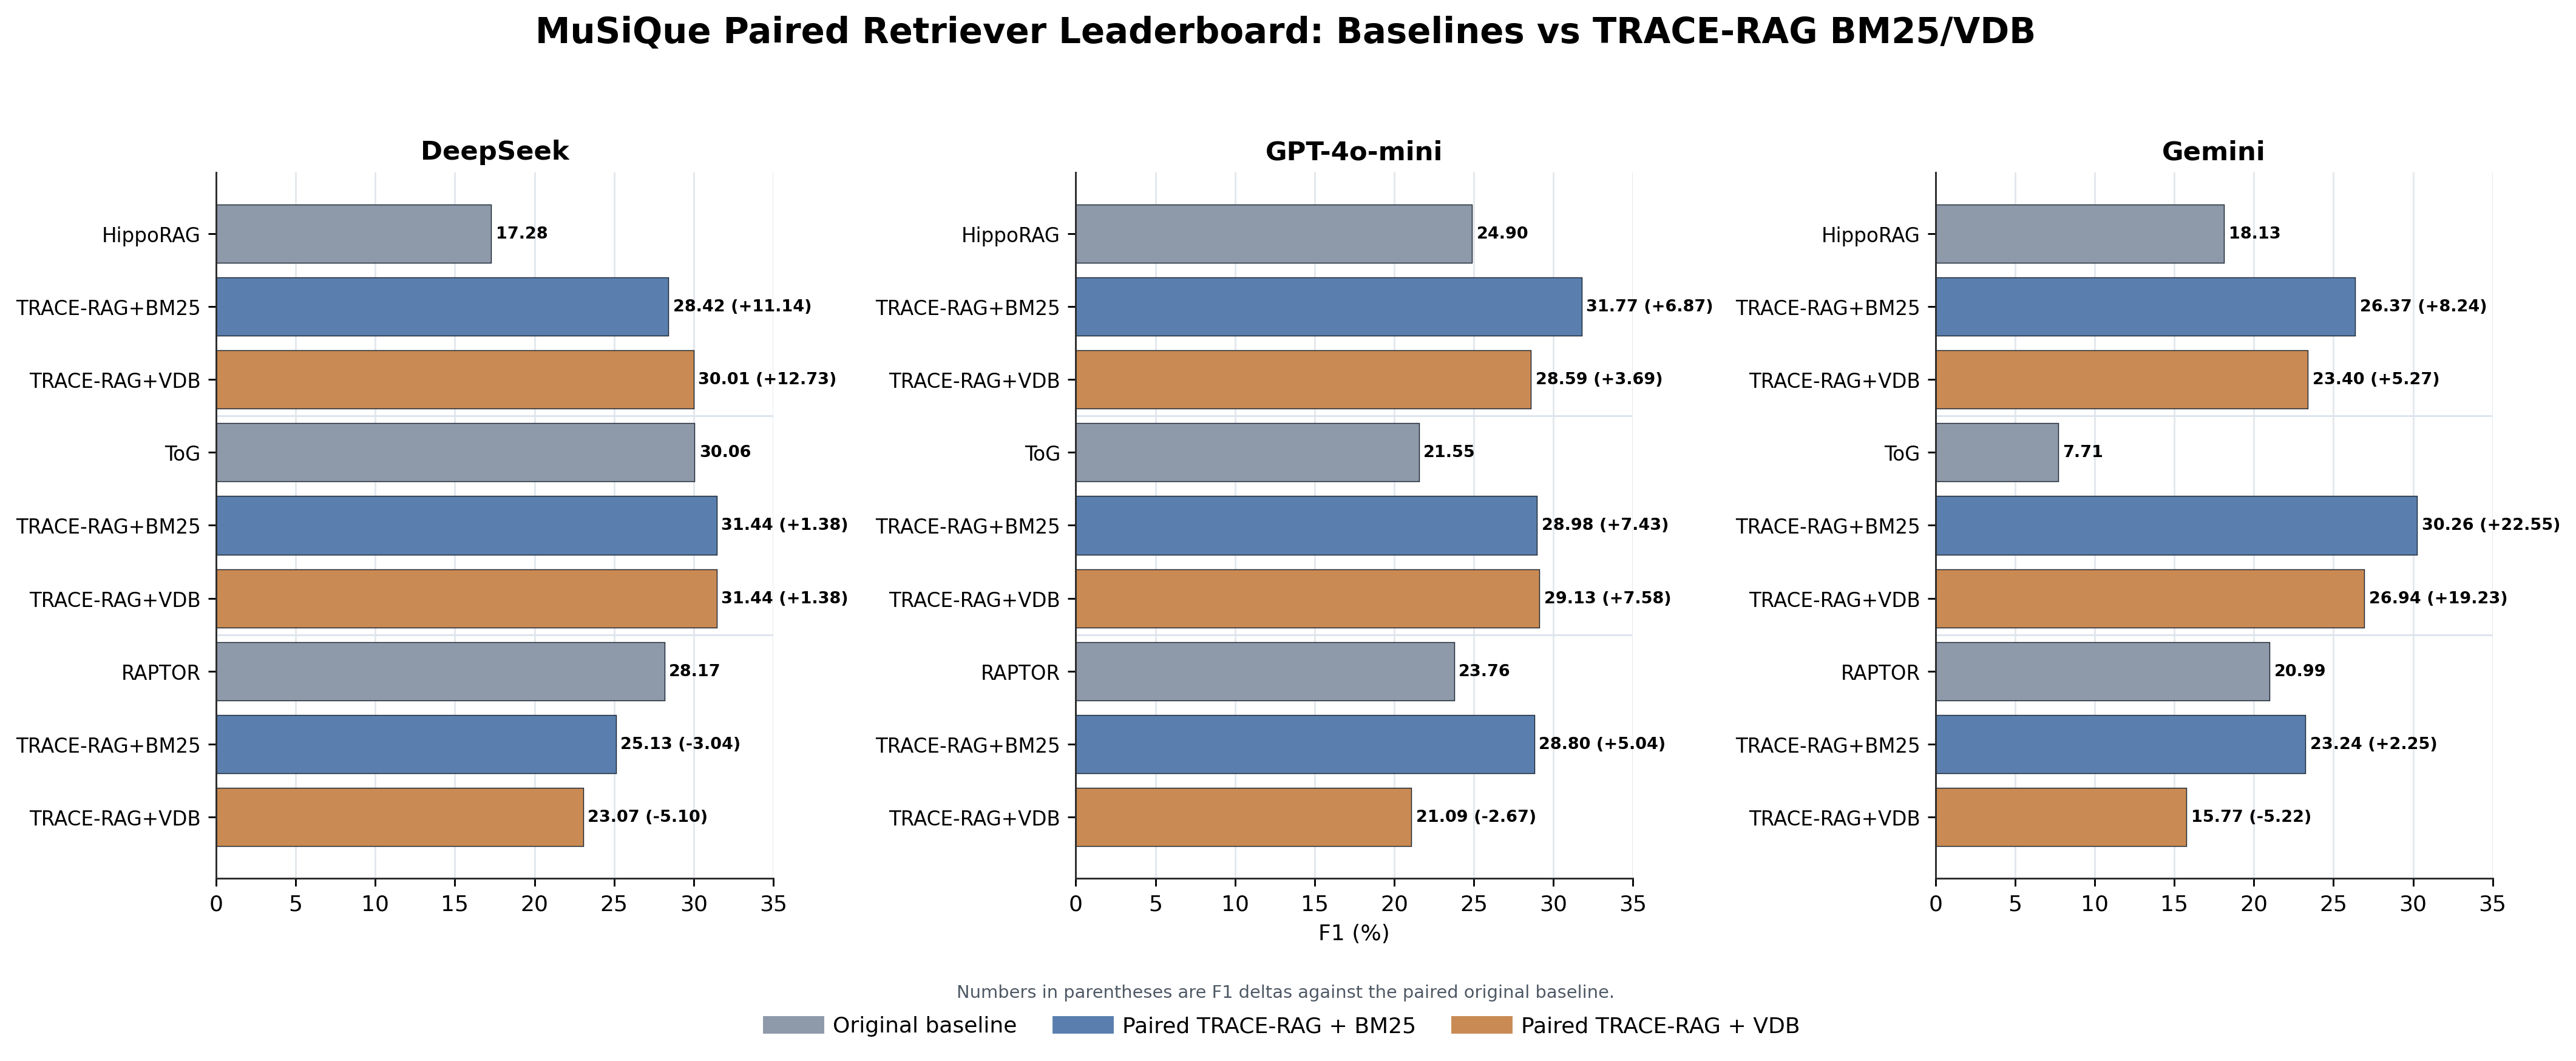
\includegraphics[width=\linewidth]{figures/positive_showcase/showcase_musique_leaderboard.png}
\caption{MuSiQue method comparison grouped by model and graph-retriever family.
Gray bars show the original graph baseline; colored bars show the paired TRACE-RAG
variants using BM25 or VDB text retrieval.}
\label{fig:musique-leaderboard}
\end{figure}

\subsection{Paired-Retriever Analysis}
\label{sec:paired-retriever-analysis}

The main-result comparison asks whether TRACE-RAG beats the strongest available
baseline. We also evaluate a paired-retriever question: does TRACE-RAG improve over
the graph retriever that supplies its graph component? Across 36 paired
comparisons, TRACE-RAG improves F1 in 25 cases, or 69.4\% of pairs. The mean change
over all pairs is +4.78 F1, and the mean gain among positive pairs is +7.67 F1.
This analysis shows that TRACE-RAG often strengthens the retriever family it is
paired with, especially when the graph-only baseline is weak or unstable.

\begin{table}[t]
\centering
\small
\begin{tabular}{lllrrr}
\toprule
Dataset & Model & Pair & Baseline F1 & TRACE-RAG F1 & $\Delta$F1 \\
\midrule
MuSiQue & Gemini & tog+bm25 & 7.71 & 30.26 & +22.55 \\
MuSiQue & Gemini & tog+vdb & 7.71 & 26.94 & +19.23 \\
PopQA & Gemini & tog+bm25 & 11.97 & 25.97 & +14.00 \\
PopQA & Gemini & tog+vdb & 11.97 & 24.71 & +12.74 \\
MuSiQue & DeepSeek & hippo+vdb & 17.28 & 30.01 & +12.73 \\
MuSiQue & DeepSeek & hippo+bm25 & 17.28 & 28.42 & +11.14 \\
\bottomrule
\end{tabular}
\caption{Largest positive paired-retriever F1 gains. Each row compares a TRACE-RAG
variant with the graph retriever baseline used by that TRACE-RAG configuration.}
\label{tab:paired-retriever-gains}
\end{table}

\begin{figure}[t]
\centering
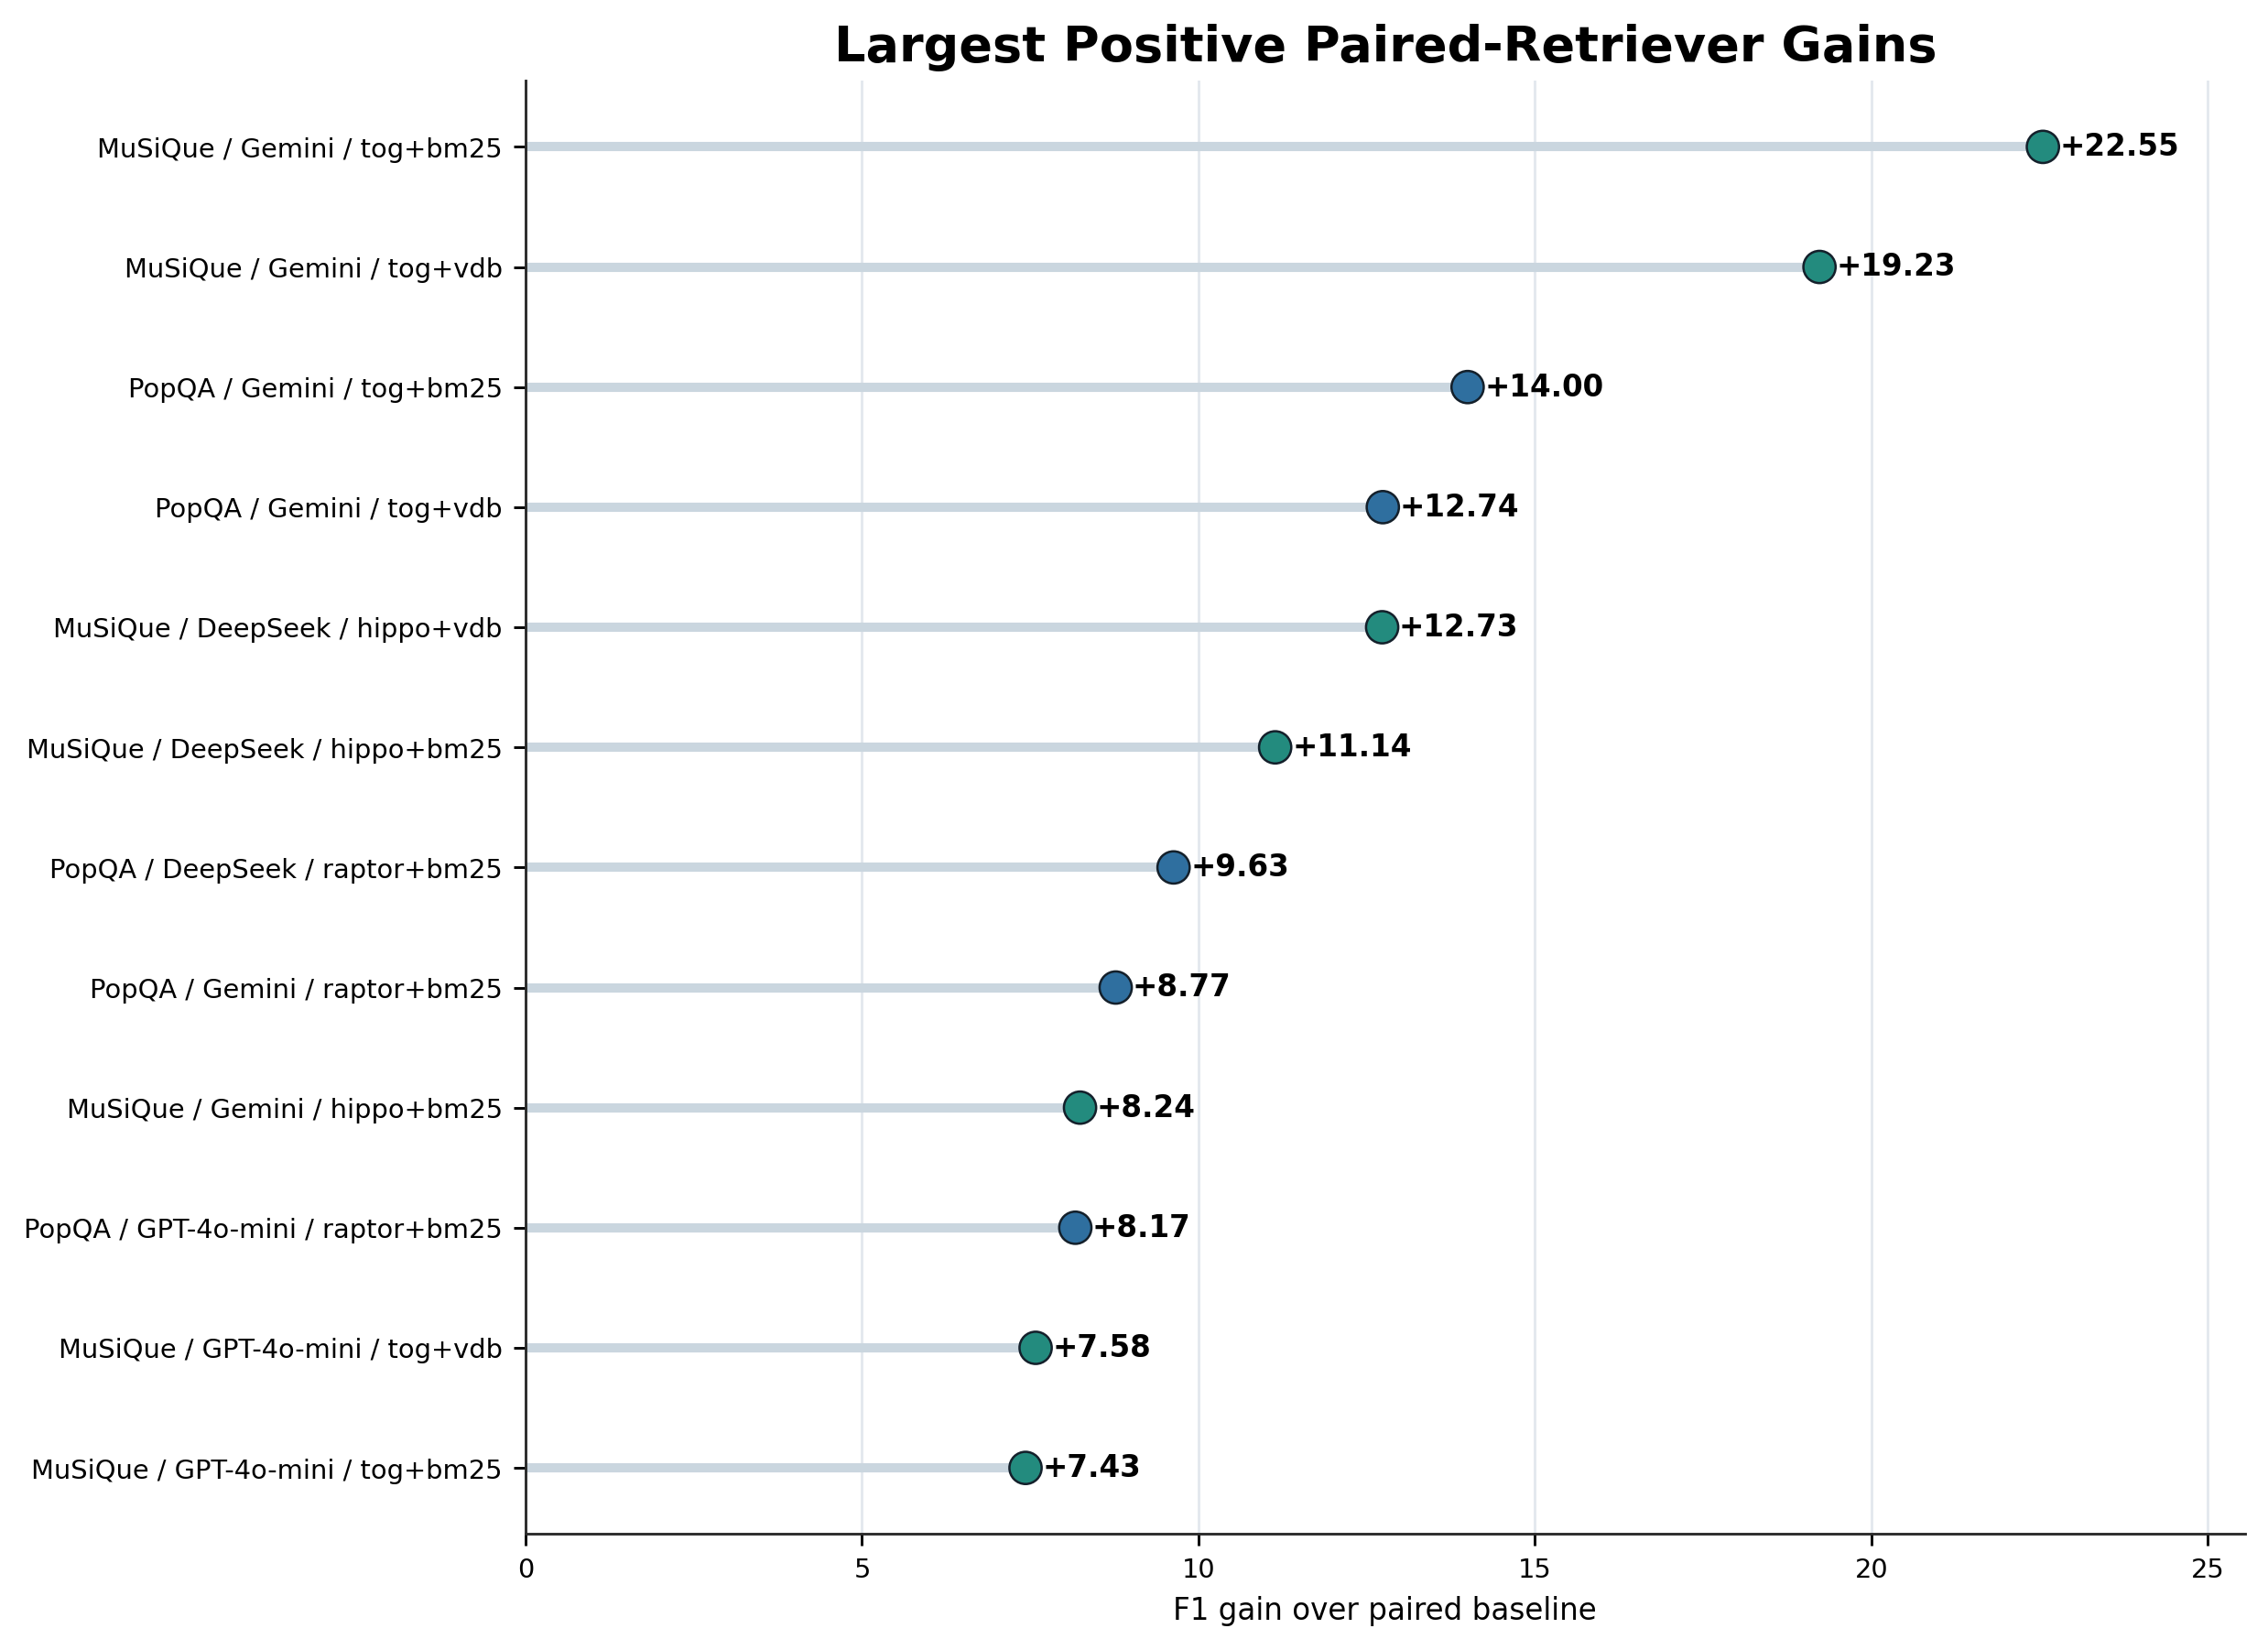
\includegraphics[width=\linewidth]{figures/positive_showcase/panel_largest_positive_paired_retriever_gains.png}
\caption{Largest positive paired-retriever F1 gains. The ranked view highlights
the strongest cases where a TRACE-RAG variant improves over the graph retriever
baseline used by its graph component.}
\label{fig:paired-retriever-largest-gains}
\end{figure}

\subsection{Ablation Study}
\label{sec:ablation-study}

The leave-one-out ablation uses Gemini with hippo+bm25 and compares the full
system with variants that remove one component at a time. We report
``Full TRACE-RAG minus ablated variant'', so positive values indicate that removing
the component hurts performance. The Critic is the most consistent component:
removing it reduces F1 on MuSiQue by 5.33 points and on PopQA by 1.04 points.
The answer normalizer is important for exact-match and precision stability,
reducing EM by 6.50 points on MuSiQue and 38.50 points on PopQA when removed.

\begin{table}[t]
\centering
\small
\begin{tabular}{llrrrrr}
\toprule
Dataset & Removed component & $\Delta$Acc. & $\Delta$EM & $\Delta$Prec. & $\Delta$Rec. & $\Delta$F1 \\
\midrule
MuSiQue & Critic & +4.50 & +4.00 & +5.37 & +5.50 & +5.33 \\
MuSiQue & Answer normalizer & -3.50 & +6.50 & +5.17 & +0.68 & +3.59 \\
PopQA & Critic & +2.50 & +2.00 & +2.25 & +0.83 & +1.04 \\
PopQA & Answer normalizer & -7.00 & +38.50 & +21.46 & -4.19 & +1.45 \\
\bottomrule
\end{tabular}
\caption{Key leave-one-out ablation effects for Gemini hippo+bm25. Values are
full-system scores minus ablated-variant scores; positive values mean the
removed component contributes positively to the metric.}
\label{tab:key-ablation-effects}
\end{table}

\begin{figure}[t]
\centering
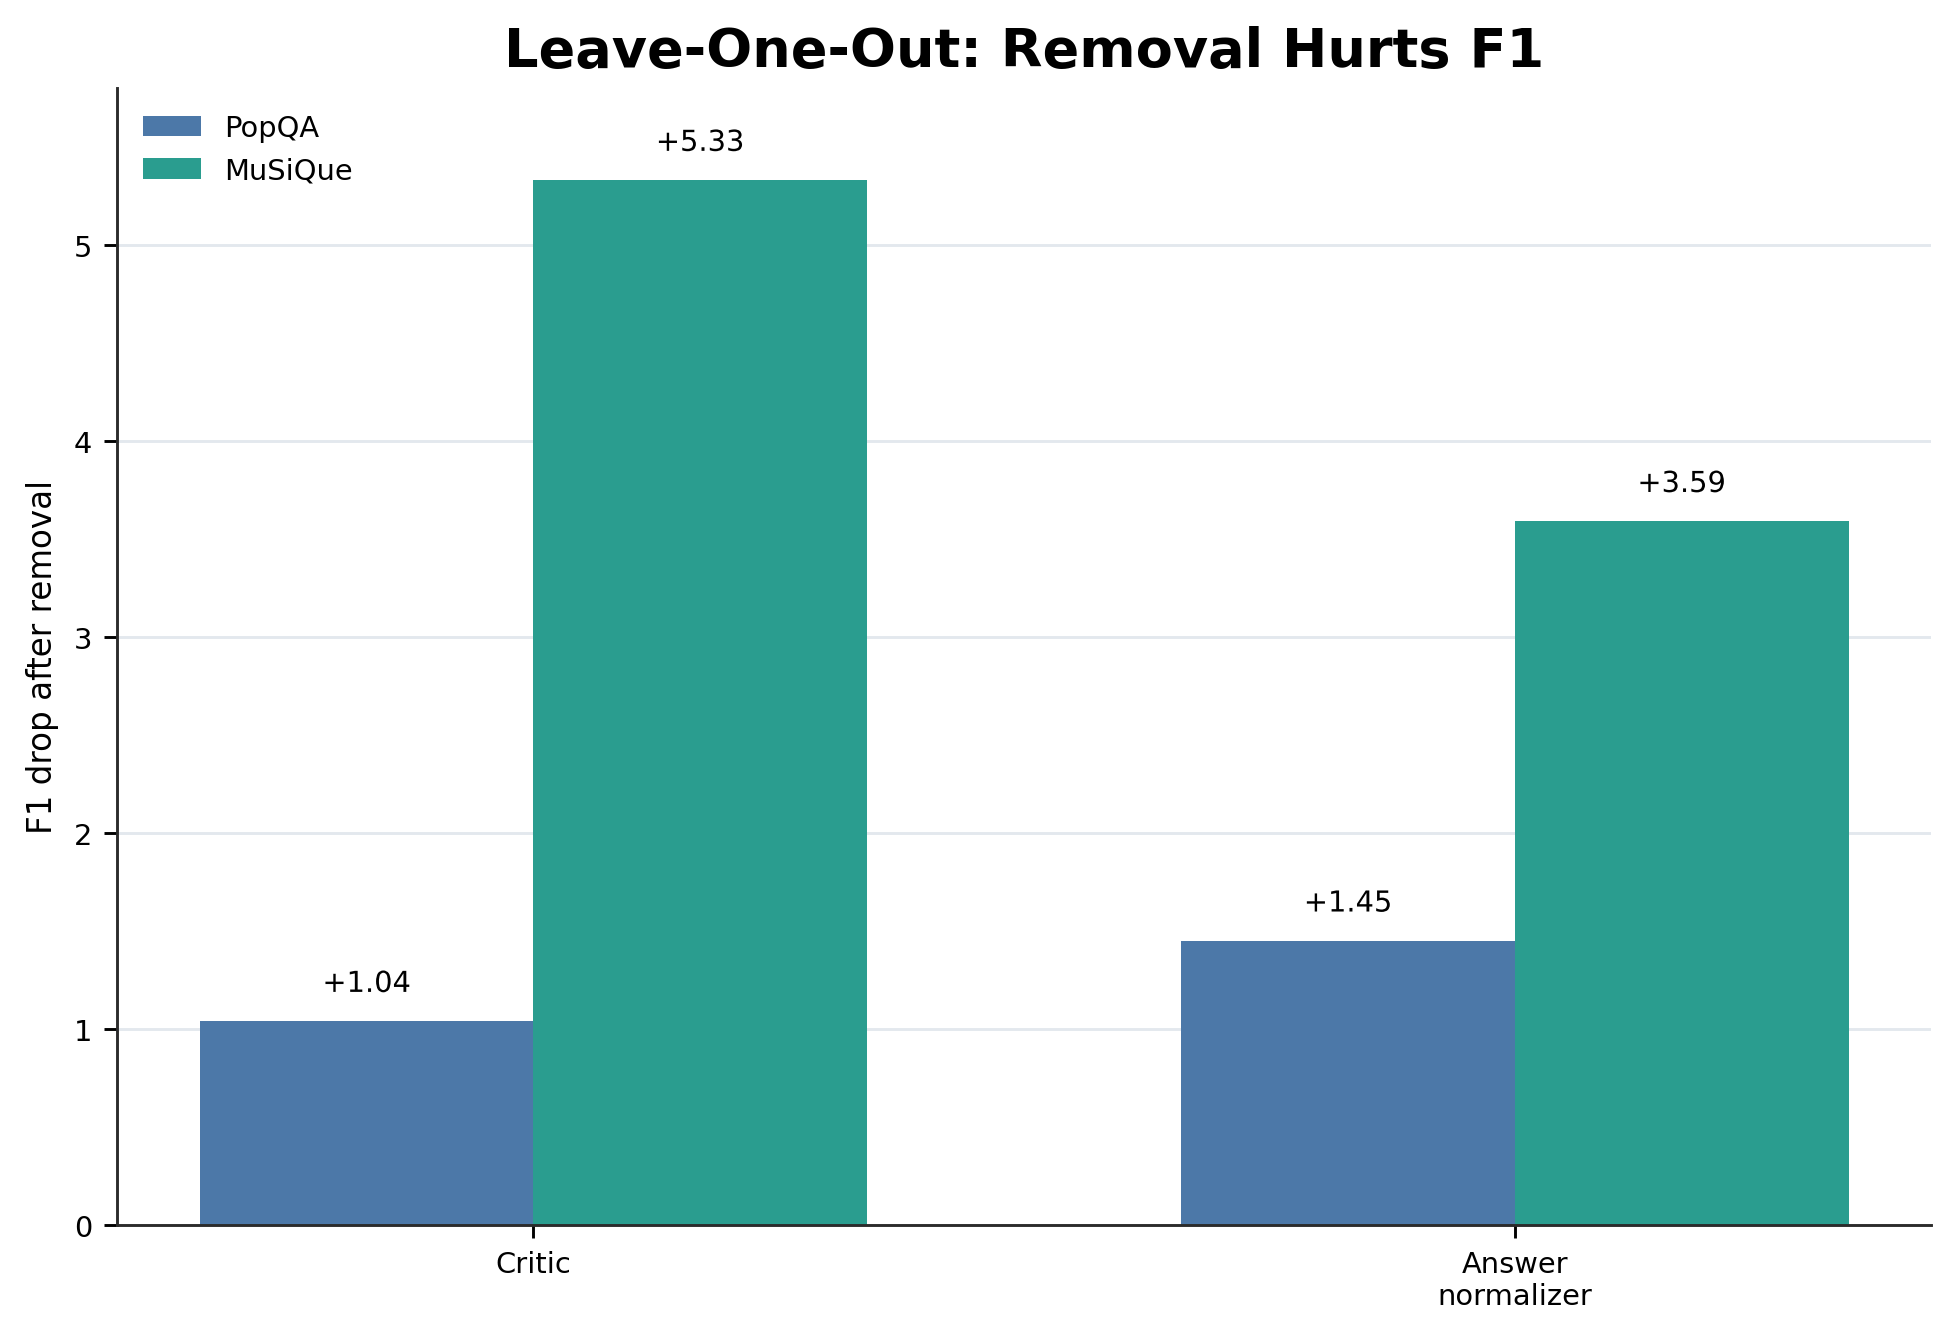
\includegraphics[width=\linewidth]{figures/positive_showcase/panel_leave_one_out_removal_hurts_f1.png}
\caption{Leave-one-out F1 effects for the most useful TRACE-RAG components. Positive
values indicate that removing the component reduces F1 relative to the full
TRACE-RAG system.}
\label{fig:leave-one-out-f1}
\end{figure}

\paragraph{Summary.}
The primary evidence for TRACE-RAG is the consistent improvement on MuSiQue across
all tested model backbones. PopQA provides a conservative robustness check:
TRACE-RAG stays close to strong factoid-QA baselines and improves several paired
retriever settings, but it should not be framed as a uniform win. The ablation
results identify the Critic and answer normalizer as the most reliable
contributors in the current setting, while other modules should be discussed as
context-dependent or moved to appendix analysis.

